\documentclass[a4, 12pt]{article}
\usepackage[a4paper, top=17mm, bottom=17mm, left=17mm, right=17mm]{geometry}
\usepackage[utf8]{inputenc}
\usepackage[T2A,T1]{fontenc}
\usepackage[colorlinks,filecolor=blue,citecolor=green,unicode,pdftex]{hyperref}
\usepackage{cmap}
\usepackage[english,russian]{babel}
\usepackage{amsmath}
\usepackage{amssymb,amsfonts,textcomp}
\usepackage{color}
\usepackage{array}
\usepackage{hhline}
\hypersetup{colorlinks=true, linkcolor=blue, citecolor=blue, filecolor=blue, urlcolor=blue, pdftitle=1, pdfauthor=, pdfsubject=, pdfkeywords=}
\usepackage[pdftex]{graphicx}
\usepackage{graphicx}
%\usepackage{literat}
\usepackage{indentfirst}
\usepackage{multirow}
\usepackage{subfig}

\sloppy
\pagestyle{plain}

\title{QReal: платформа визуального предметно-ориентированного моделирования}

\author{А.Н.Терехов \and Т.А.Брыксин \and Ю.В.Литвинов}
\date{}
\begin{document}

\maketitle
\thispagestyle{empty}

\begin{quote}
\small\noindent
В статье описывается подход к разработке программного обеспечения, основанный на специализированных графических языках. Рассматриваются существующие платформы для создания специализированных визуальных сред разработки, описывается платформа QReal, разрабатываемая на кафедре системного программирования СПбГУ, дается описание общей архитектуры системы, основных ее функциональных особенностей, приводятся примеры ее практического применения.
\end{quote}

\section*{Введение}

Разработка больших программных систем --- непростая задача. Связано это, в частности, с тем, что программное обеспечение нематериально и невидимо, его трудно представить себе визуально, а держать в голове сотни тысяч строк программного кода одновременно невозможно. Бороться с этой проблемой призвано визуальное моделирование --- подход, при котором программа представляется в виде набора моделей на графических языках, описывающих систему с различных точек зрения, от требований до описания деталей реализации. Визуальное моделирование активно применяется сейчас при анализе и проектировании, но в подавляющем большинстве случаев визуальные модели используются только как часть технической документации и как средства передачи информации программистам, тогда как было бы полезнее автоматически генерировать код системы по визуальным моделям.

В случае с визуальными языками общего назначения полноценное создание системы с использованием только графических языков чрезвычайно сложно по ряду причин, основной из которых является семантический разрыв между моделями и кодом~\cite{koznov}. Однако же, зачастую оказывается, что можно создать свой визуальный язык под конкретную предметную область или даже конкретную задачу, и, используя знания о предметной области при разработке инструментария для этого языка, добиться полной генерации работающего исходного кода системы по визуальным моделям. При этом сами модели могут оставаться достаточно близкими к предметной области, чтобы их могли создавать и использовать даже непрограммисты. Такой подход называется предметно-ориентированным визуальным моделированием (Domain-Specific Modelling, DSM), и результаты ряда исследований~\cite{dsm2, dsm3, dsm1} указывают на то, что он оказывается весьма эффективным: отмечается повышение эффективности труда программиста от трёх до десяти раз.

Разумеется, создание визуального языка, редакторов, генераторов и других инструментов для этого языка “с нуля” под каждую конкретную задачу было бы неоправданно трудоёмким. Поэтому существуют инструменты, позволяющие в большой степени автоматизировать этот процесс, такие инструменты называются DSM-платформами или metaCASE-системами. Такие системы позволяют создавать визуальную технологию (называемую DSM-решением) за время порядка дней, что делает это экономически оправданным даже для небольших проектов. Существуют зрелые коммерческие и исследовательские DSM-платформы (например, MetaEdit+, Eclipse GMP), но предметно-ориентированное моделирование применяется всё ещё довольно редко. Это связано, в частности, с недостатками существующих DSM-платформ и отсутствием методологической базы для их применения, что говорит о необходимости вести дальнейшие исследования в этой области.

Один из исследовательских проектов в области предметно-ориентированного моделирования, QReal~\cite{qreal2, qreal1}, ведётся на кафедре системного программирования Санкт-Петербургского государственного университета с 2007 года и базируется на более чем двадцатилетнем опыте коллектива кафедры в разработке графических языков~\cite{rtst1, rtst2, rtst4, rtst3, asu, rtst5}. Проект ставит перед собой цель создания DSM-платформы, достаточно простой в использовании, чтобы свой визуальный язык в течение нескольких часов мог создать даже человек, который использует её впервые, и при этом достаточно функциональной, чтобы с её помощью можно было разрабатывать большие и сложные визуальные технологии\footnote{Домашняя страница проекта QReal на GitHub, URL: \url{https://github.com/qreal/qreal}}. О текущих результатах этого проекта и пойдёт речь в данной статье.

\section{Существующие DSM-платформы}

На данный момент существует несколько известных DSM-платформ, таких как Eclipse Graphical Modeling Project, MetaEdit+, Visual Studio Visualization and Modeling SDK (ранее называвшийся Microsoft DSL Tools) и большое число академических разработок. 

Graphical Modeling Project\footnote{Graphical Modeling Project homepage, URL: \url{http://www.eclipse.org/modeling/gmp/}} \footnote{Более подробный обзор на русском языке см. в~\cite{emp}} --- набор проектов, разрабатываемых в рамках проекта с открытым исходным кодом Eclipse, связанных с разработкой редакторов визуальных языков. Наиболее зрелыми проектами из этого направления являются библиотеки Graphical Editing Framework (GEF) и Eclipse Modeling Framework (EMF). GEF --- это средство для создания векторных графических редакторов, обладающих широкими возможностями взаимодействия с пользователем. EMF --- это средство для генерации классов модели и инструментальной поддержки для визуальных языков по метамоделям\footnote{Метамодель --- модель, описывающая синтаксис визуального языка}, представленным в различных форматах (XMI\footnote{XML Metadata Intercharge, стандарт хранения визуальных моделей, см. \url{http://www.omg.org/spec/XMI/2.4.1/}}, аннотированных Java-классов, и других). Цель проекта GMP --- 
объединить эти и ряд других технологий в единую DSM-платформу на базе среды разработки Eclipse.

На данный момент GMP стал стандартом де-факто для научных исследований, связанных с визуальним моделированием и метамоделированием. Однако этот проект плохо подходит для промышленного использования, потому как на данный момент находится в стадии активного развития. Постоянно вносятся изменения, документация либо отсутствует, либо устарела. Кроме того, GMP состоит из довольно слабо связанных между собой компонентов, развивающихся независимо, и целостной технологии, поддерживающей весь цикл разработки визуального языка, пока не создано. Это приводит к довольно большой сложности разработки в рамках GMP и высокому порогу вхождения --- для создания даже простого языка требуется строить несколько моделей (модели абстрактного и конкретного синтаксисов языка\footnote{Абстрактный синтаксис отвечает за логическую структуру модели, конкретный --- за её внешний вид. Определение этих и других базовых понятий метамоделирования см. в~\cite{koznov}}, модель инструментов, где описываются пункты меню и подобные вещи, модель 
соответствия между этими моделями и т.д.). Поэтому потребность в создании исследовательских DSM-платформ “с нуля” всё-таки есть, и такие платформы существуют (и продолжают появляться) несмотря на наличие GMP.

DSM-платформа MetaEdit+\footnote{DSM-платформа MetaEdit+, URL: \url{http://www.metacase.com/}} является на сегодняшний день самой зрелой и активно используется организациями-разработчиками программного обеспечения. Платформа развилась из академической разработки MetaEdit, превратившись в коммерчески успешный проект. MetaEdit+ позволяет задавать метамодели визуальных языков с использованием визуального метаязыка GOPPRR (аббревиатура, образованная основными сущностями метаязыка --- graph, object, property, port, role, relationship). В состав платформы входит графический редактор для задания внешнего вида сущностей создаваемого языка, и набор средств для описания правил генерации кода по визуальным моделям. Сами правила задаются в текстовом виде на специальном языке, есть возможность вызывать одни правила из других, связь между правилами задаётся в графическом виде.

Несмотря на то, что авторы MetaEdit+ активно публикуют свои научные результаты (см., например, книгу~\cite{dsmbook}), исходные коды системы закрыты, а сама система стоит весьма дорого. Это делает невозможным в полной мере переиспользовать опыт проекта MetaEdit+ и реализовывать на его основе новые возможности. 
	
Система Visual Studio Visualization and Modeling SDK (VMSDK)\footnote{Visual Studio Visualization and Modeling SDK (бывший DSL SDK), URL: \url{http://archive.msdn.microsoft.com/vsvmsdk}}, ранее Microsoft DSL Tools --- расширение для среды разработки Microsoft Visual Studio, позволяющее генерировать редакторы визуальных языков в виде подключаемых модулей для Visual Studio. Метамодель языка задаётся в графическом виде, с ней связывается внешний вид элементов языка. Внешний вид элемента можно выбирать из фиксированного числа геометрических фигур, либо задать произвольную иконку. Если требуется использовать какое-то нестандартное отображение элемента (например, не прямоугольник, а ромб), требуется ручное кодирование на языке C\#. Несмотря на то, что система VMSDK распространяется бесплатно, ни она сама, ни сгенерированные с её помощью редакторы не могут работать вне среды Visual Studio, которая стоит весьма дорого и имеет закрытые исходные коды.

Таким образом, существует необходимость разработки DSM-платформ для исследовательских целей, проект QReal --- одна из таких разработок.

\section{Проект QReal}

Изначально проект QReal был посвящен созданию среды моделирования, включающей в себя набор редакторов UML 2.0, однако требуемые редакторы по функциональности были слишком похожи друг на друга, чтобы создавать их друг за другом кодированием “вручную”. Возникла необходимость в средствах быстрого создания визуальных языков и инструментальной поддержки для них.

Для автоматизации процесса создания таких редакторов метамодели соответствующих языков (внешнего вида и свойств элементов языка и связей между этими элементами) должны быть описаны формально с помощью некоторого языка\footnote{В случае текстовых языков для этого чаще всего используются формы Бэкуса-Наура}, текстового или графического (или даже набора языков). Далее эти описания могут быть использованы следующим образом:

\begin{itemize}
 \item в рамках генеративного подхода по описанию метамодели генерируется программный код, который тем или иным образом дополняет код самого DSM-решения, привнося в него особенности данного языка;
 \item в рамках интерпретативного подхода в состав DSM-решения входит механизм, который по запросу читает нужные данные прямо из описания метамодели и обрабатывает их нужным образом (например, считывает количество и тип свойств элементов и отображает их в редакторе свойств). То есть во время работы с редактором происходит интерпретация метамодели языка.
\end{itemize}

Первый подход более прост в реализации и обычно дает определенный выигрыш в скорости работы, однако второй позволяет создавать более гибкие инструменты --- например, позволяет менять метамодель языка динамически в процессе работы с редактором этого языка.

Исторически в QReal первым был реализован генеративный подход, что сделало архитектуру инструмента как можно более модульной (см. рис.~\ref{fig1}) --- конкретные DSM-решения на основе QReal получаются дополнением и параметризацией кода самой DSM-платформы. Абстрактная функциональность редакторов (например, такая, как способность двигать и масштабировать элементы на диаграммах, соединять их связями, хранить в репозитории значения их свойств и т.п.) максимально абстрагируется и формирует так называемое ``ядро'' системы, в то время как специфика каждого конкретного визуального языка оформляется в виде подключаемого модуля-плагина. Код каждого такого модуля генерируется автоматически по описанию метамодели языка, компилируется в плагин и не зависит от каких-либо других частей QReal. Плагины загружаются диспетчером модулей, который, в свою очередь, предоставляет интерфейс остальным частям QReal для доступа к информации, содержащейся в плагинах редакторов --- именам и типам элементов и связей между ними, 
изображениям элементов, числу и типу их свойств, правилам соединения элементов связями и т.п.

\begin{figure} [ht]
  \begin{center}
    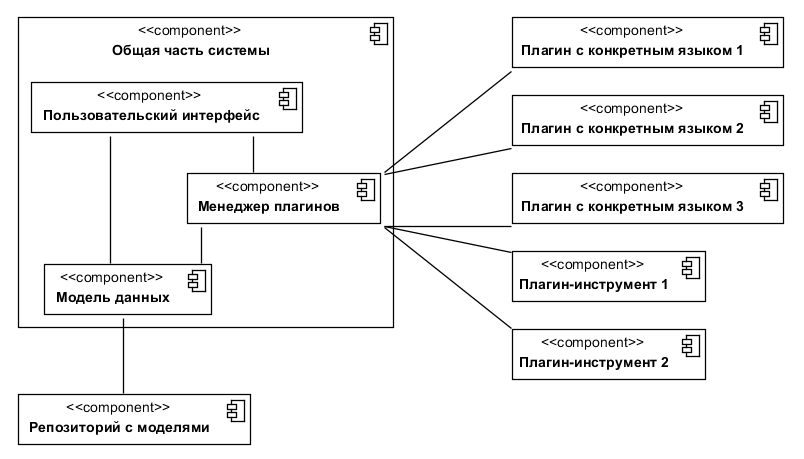
\includegraphics[width=0.9\textwidth]{fig1-architecture-overview.png}
    \caption{Общая архитектура DSM-решений на основе QReal}
    \label{fig1}
  \end{center}
\end{figure}

Помимо плагинов редакторов в QReal существуют также плагины инструментов. В них выносится функциональность различных инструментальных средств CASE-пакета, которые могут быть полезны проектировщику --- механизм версионирования моделей, генераторы кода, отладчики и интерпретаторы, механизм задания и проверки ограничений на создаваемые модели, механизм задания и проведения рефакторингов моделей и т.п. 

Это позволяет максимально переиспользовать инструменты между создаваемыми на базе QReal DSM-решениями --- стоит добавить какую-нибудь функциональность в ``ядро'' системы или оформить ее в отдельный подключаемый модуль, и все DSM-решения при желании получат эту функциональность автоматически. 

\section{Средства метамоделирования}

Для описания метамодели разрабатываемого языка в QReal применяется два подхода:
\begin{itemize}
 \item \textit{графический:} метамодель задается разработчиком языка графически в метаредакторе QReal с помощью простого визуального языка, являющего аналогом MOF\footnote{MetaObject Facility, URL: \url{http://www.omg.org/mof/}}. Для описания представлений элементов языка на диаграммах используется графический редактор форм, позволяющий либо создавать новые векторные изображения из набора примитивов, либо загружать уже готовые растровые.
 \item \textit{текстовый:} метамодель описывается с помощью XML-формата, графические изображения элементов задаются на разработанном нами языке WTF (widget template format), являющимся расширением языка описания векторной графики SVG~\footnote{Scalable Vector Graphics, URL: \url{http://www.w3.org/Graphics/SVG/}}.
\end{itemize}

Стоит отметить, что в QReal эти два подхода являются взаимозаменяемыми, поскольку XML-описание метамодели языка может быть как загружено в метаредактор, так и сгенерировано из него. Исторически в QReal текстовый способ задания метамоделей появился раньше, однако в настоящее время графический метаредактор используется чаще как более выразительное средство.

Типичный процесс создания нового языка в QReal проходит следующим образом. Используя метаредактор, автор языка создает модель, описывающую желаемый язык --- определяет сущности этого визуального языка и связи между ними (в метаязыке им соответствует блоки ``Элемент'' и ``Связь''). Также с помощью метаредактора можно задавать отношения наследования между элементами на диаграмме и отношения допустимой вложенности одних элементов в другие как в контейнеры. Эти отношения на диаграмме указываются направленными ассоциациями. Помимо этого имеется возможность задавать некоторые дополнительные свойства создаваемого графического редактора, поддержка которых осуществлена в “ядре” QReal (способность «вытягивать» из элементов определенные связи, сортировать вложенные элементы и уметь их скрывать для элементов-контейнеров и некоторые другие).

Помимо абстрактного синтаксиса важно уметь задавать, как будут внешне выглядеть элементы разрабатываемого языка. Для этого в QReal реализован редактор формы фигур, который представляет собой по сути векторный графический редактор, но обладает рядом особенностей, отражающих специфику его использования. Например, есть возможность задания положения элементов управления, отображаемых на фигуре, позволяющих изменять свойства элемента. Это делает возможным отображение и редактирование логических свойств прямо на диаграмме при моделировании с помощью этого языка --- например, отредактировать имя элемента прямо на диаграмме или выбрать значение свойства перечислимого типа из выпадающего списка.

В QReal для разработанного метаязыка была создана инструментальная поддержка и соответствующая инфраструктура, обеспечивающие сквозной процесс создания графических редакторов: разработчик может спроектировать новый визуальный язык, скомпилировать подключаемый модуль соответствующего графического редактора и подключить его к QReal, не выходя из системы. 

Также существует набор дополнительных инструментов, позволяющих расширить функциональность создаваемых DSM-решений. 

\begin{itemize}
 \item Средства описания исполнимой семантики позволяют задавать операционную семантику для элементов динамических языков, что позволяет автоматически создавать для них в QReal визуальные интерпретаторы и отладчики.
 \item Средства задания ограничений позволяют задавать условия, которые должны выполняться применительно к элементу или группе элементов на диаграмме. Например, для элемента ``Начало'' диаграммы деятельности UML можно было бы задать, что в него не должно входить никаких связей, а исходить должна только одна. При использовании получившегося редактора данные ограничения будут проверяться автоматически на создаваемых моделях, при необходимости выдавая предупреждения и сообщения об ошибках.
 \item Средства задания рефакторингов позволяют описывать трансформации графов моделей, которые в дальнейшем могут быть выполнены при моделировании с помощью данного языка. Это могут быть общие для всех языков рефакторинги (например, выделение части диаграммы в поддиаграмму) или специфичные именно для данного языка (например, ``Выделение интерфейса'' для диаграммы классов UML).
\end{itemize}

Кроме того, в QReal реализована технология быстрого прототипирования визуального языка прямо в процессе моделирования, так называемое ``метамоделирование на лету''. При первоначальном анализе предметной области, когда визуального языка ещё нет и непонятно, какие в нём могут быть сущности и связи, диаграммы обычно рисуются в виде набросков на бумаге. ``Метамоделирование на лету'' позволяет рисовать такие наброски в CASE-системе, уточняя и формализуя визуальный язык в процессе рисования. QReal в режиме метамоделирования на лету позволяет в процессе рисования диаграммы добавлять и удалять элементы в палитре, менять их свойства и внешний вид без метаредактора. С точки зрения пользователя процесс создания визуального языка выглядит как добавление нового узла в палитру, задание его внешнего вида (если надо, иначе по умолчанию он будет рисоваться прямоугольником, что для первых набросков оказывается достаточно), определение некоторых его свойств, использование его на диаграмме, редактирование элемента и его свойств 
по результатам использования. Получившийся метаязык можно сохранить и открыть потом в метаредакторе, чтобы доопределить для него дополнительную функциональность, недоступную в режиме метамоделирования на лету, например, ограничения, правила рефакторингов, наследование и отношения вложенности между узлами. Таким образом, первые этапы разработки визуального языка в значительной степени автоматизируются, и их результаты не теряются, а, постепенно уточняясь, становятся полноценным визуальным языком.

\section{Средства моделирования}

Получаемое типовое предметно-ориентированное решение на базе QReal включает в себя следующие инструменты:

\begin{itemize}
\item графический пользовательский интерфейс, включающий в себя обозреватель модели, редактор свойств элементов, рабочую область редактора диаграмм, палитру доступных для моделирования элементов, окно для отображения предупреждений и сообщений об ошибках, а также набор меню и панелей главного окна для управления остальными инструментами;
\item репозиторий, представляющий собой простую объектно-ориентированную базу данных, хранящий все создаваемые в QReal модели.  Репозиторий представлен в виде отдельной динамически загружаемой библиотеки, в результате чего может быть использован сторонними программами (например, генераторами кода или анализаторами моделей) через специальный программный интерфейс;
\item средства для работы с логическими и графическими моделями. Логическая модель системы отражает её внутреннюю структуру, и это то, с чем работают генераторы и другие инструменты. Графическая модель системы --- это набор диаграмм, отображающих её логическую модель, с ней работает пользователь;
\item средства многопользовательской работы, основанные на версионировании создаваемых моделей. Реализованы традиционные операции систем контроля версий (сохранение и получение данных с удаленного сервера, переключения между версиями), а также возможность визуального сравнения версий одной и той же модели;
\item пошаговые отладчики и интерпретаторы, созданные либо с помощью описания семантики элементов языка при метамоделировании, либо закодированные ``вручную'' разработчиком языка;
\item генераторы кода и других артефактов по визуальным моделям. Пока в QReal отсутствуют средства быстрого автоматизированного создания генераторов кода, поэтому вся работа по созданию генераторов ложится на автора языка;
\item механизм осуществления рефакторингов, позволяющий осуществлять преобразования моделей, заданные разработчиком языка на фазе метамоделирования, а также общие для всех языков (например, переименование элементов по шаблону или выделение в поддиаграмму);
\item механизм проверки ограничений, который автоматически проверяет правила, заданные на экземпляры элементов на диаграммах (например, проверка, что значение определенного свойства входит в определенный диапазон, или что из элемента не исходит больше связей, чем задано);
\item механизм распознавания жестов мышью~\cite{qreal3}, используемый для быстрого создания элементов на диаграммах и связей между ними. Так, при создании редактора каждому элементу ставится в соответствие отдельный жест мышью, и если в процессе моделирования разработчик зажмет правую кнопку мыши и сделает похожий жест, на диаграмме появится соответствующий элемент. Связь между элементами можно создать, осуществив жест мышью, начинающийся и заканчивающийся на интересующих элементах на диаграмме.
\end{itemize}

Все описанные инструменты реализованы в виде подключаемых модулей, поэтому по необходимости выбранное DSM-решение может быть сконфигурировано произвольным их числом. Это бывает полезно, поскольку если стоит цель в создании легковесного редактора (например, для целей обучения), отладчики или рефакторинги моделей его только усложнят.

В последнее время в проекте QReal довольно много внимания уделяется вопросам удобства использования средств визуального моделирования и удобству самого процесса моделирования в частности. Одни из самых частых операций при моделировании --- это создание и удаление элементов и связей на диаграммах, а также ``красивое'' расположение их относительно друг друга. Автоматизируя или упрощая эти операции, можно сократить время и число рутинных операций проектировщика, облегчив его работу. В этом направлении помимо рассмотренного распознавания жестов мышью был реализован еще один способ быстрого создания связей --- при выделении объекта на диаграмме вокруг него появляются несколько вспомогательных графических элементов (в форме разноцветных кружков), каждый из которых ассоциирован с видами связей, которые из данного элемента могут исходить. При нажатии на них из элемента можно ``вытащить'' связь. Если пользователь при этом отпускает кнопку мыши на свободном пространстве диаграммы, ему предлагается список элементов, 
которых можно соединить с выбранным данным типом связи. Если же кнопка мыши отпускается на существующем элементе, система проверяет, можно ли соединить эти элементы выбранным типом связи, и решает, стоит ли создавать данную ассоциацию или нет. 

Также в этом направлении было сделано много мелких улучшений, таких как средства автоматической раскладки элементов на диаграмме, режим ``перпендикулярных связей'' (связи задаются ломаными линиями, участки которых соединяются между собой под прямым углом), а также ряд эвристик языка ДРАКОН~\cite{dragon} --- создание групп элементов, возможность вставки элемента ``внутрь'' связей и некоторые другие.

\section{Апробация}

Самой успешной на данный момент визуальной предметно-ориентированной технологией, созданной с помощью QReal, является QReal:Robots~\cite{qrealrobots} --- средство программирования роботов Lego Mindstorms NXT 2.0\footnote{LEGO Mindstorms homepage, URL: \url{http://mindstorms.lego.com/en-us/Default.aspx}}. Ситуация, в которой появился этот проект, весьма типична для предметно-ориентированного моделирования --- есть достаточно узкая предметная область, потребность в нетривиальных средствах программирования в этой предметной области и DSM-платформа, позволяющая быстро создать нужные средства программирования.

\subsection{Постановка задачи}

Изучение информатики в школах базируется на понятии “исполнителя” --- некоторого объекта, который выполняет команды, описанные в программе, в некотором окружении. В качестве такого исполнителя до сих пор активно применяется ``черепашка'' LOGO\footnote{См., например, MyRobot, Язык программирования Лого, URL: \url{http://myrobot.ru/logo/aboutlogo.php}}, но она постепенно вытесняется робототехническими конструкторами, в частности, Lego Mindstorms NXT, которые имеют ряд преимуществ. Прежде всего, они материальны, кроме того, они имеют датчики, с помощью которых могут “видеть” внешнюю среду, к тому же, детям интересно собирать из конструктора робот, который они потом будут программировать. Существуют методические пособия по преподаванию информатики с использованием этого конструктора в школах, например,~\cite{lego}.

Программировать такие роботы, однако же, сложно, потому как из одного набора деталей можно собрать самые разные конструкции, так что базовым набором команд будут не команды вида ``вперёд на 20 шагов'', ``влево на 90 градусов'', как в ``черепашке'', а низкоуровневые команды вида ``мотор, подключенный к порту А, включить с мощностью 70\% на 3 полных оборота''. Поэтому для обучения школьников 5-6 классов программированию обычно используются визуальные среды Robolab~\cite{robolab} и NXT-G\footnote{LEGO web site, NXT-G download page, URL: \url{http://service.lego.com/en-us/helptopics/?questionid=2655}}, где программа представляет собой набор блоков, каждый из которых представляет элементарную команду роботу. Такие программы гораздо нагляднее кода на языках типа C.

Существующие визуальные среды имеют ряд недостатков с точки зрения преподавания в школах, настолько существенных, что есть насущная потребность в создании новой визуальной среды. Такой средой и должна стать система QReal:Robots. С научной точки зрения она интересна тем, что создавалась с помощью QReal и является хорошим примером визуальной технологии, созданной с помощью DSM-платформы, которая дошла до фазы практического внедрения.

\subsection{Функциональность системы QReal:Robots}

Концептуально программа на языке QReal:Robots представляется в виде набора элементарных команд роботу, связанных стрелками, означающими передачу управления между блоками. Пример программы представлен на рис.~\ref{fig2}.

\begin{figure} [ht]
  \begin{center}
    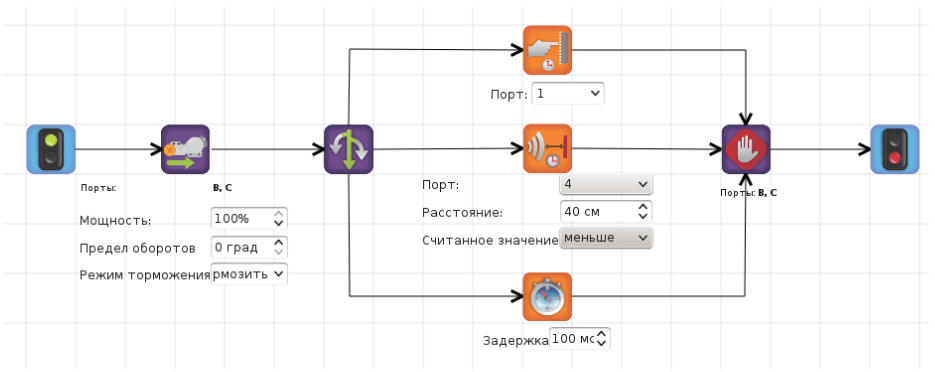
\includegraphics[width=1.0\textwidth]{fig2-qreal-robots.png}
    \caption{Пример программы в QReal:Robots}
    \label{fig2}
  \end{center}
\end{figure}

Созданную на визуальном языке программу можно исполнить прямо на компьютере, посылая команды роботу через Bluetooth или USB. При этом текущий исполняемый блок будет подсвечиваться, будут выводиться показания сенсоров и значения переменных и будет возможность остановить или даже изменить программу в процессе выполнения. По диаграмме также можно сгенерировать код на языке C для операционной системы nxtOSEK\footnote{nxtOSEK --- операционная система реального времени, работающая на роботах NXT и совместимая со стандартной прошивкой. Является самой быстрой на данный момент ОС для NXT. Более подробно см. \url{http://lejos-osek.sourceforge.net/}}, загрузить его на робот и исполнить на роботе. При этом отладочная информация выводиться не будет, но робот будет способен действовать автономно, без связи с компьютером. Кроме того, программу можно исполнить вообще без робота, на двухмерной модели, запущенной внутри среды QReal:Robots. Двухмерная модель реализует фиксированную конфигурацию робота (трёхколёсную тележку, 
типичную для задач, требующих перемещения робота в пространстве, например движения по линии или игре в робофутбол), но есть возможность задать конфигурацию и положение сенсоров, элементы внешнего мира: стены, цветные линии и области на полу. 

Визуальный язык состоит из порядка двадцати блоков и одного вида связи, поддерживает математические выражения с арифметическими операциями и тригонометрическими функциями, использование переменных, доступ к текущим значениям сенсоров прямо из выражения. Есть поддержка параллельно исполняемых фрагментов программы, условного оператора и циклов. 

\subsection{Использование DSM-платформы QReal при разработке QReal:Robots}

Наиболее полезной DSM-платформа оказалась при разработке визуального языка и редактора для него. Первый прототип языка был создан в течение нескольких часов, причём большую часть времени занял поиск подходящих иконок для блоков. Визуальный язык создавался в метаредакторе QReal. Метамодель языка активно использовала такие возможности метаязыка, как наследование (например, в иерархии “абстрактный блок” -- “блок управления двигателем” -- “блок управления мощностью” -- “моторы вперёд”/”моторы назад”), задание перечислений, использование нескольких образов одного логического элемента метамодели на диаграмме (узел “абстрактный блок” был использован в метамодели дважды, поскольку от него наследуются остальные блоки и обилие входящих в него связей “наследование” загромождало бы диаграмму). Первый работающий прототип системы был представлен кибернетикам через неделю после начала разработки и включал в себя язык и интерпретатор, управлявший роботом по Bluetooth.

QReal не смог помочь при написании интерпретатора диаграмм, код интерпретатора пришлось писать вручную. QReal при этом использовался только в виде репозитория, откуда бралась информация о диаграммах. Сам интерпретатор был написан вручную на $С++$. Это вполне закономерно, поскольку интерпретатор включает в себя код, сильно связанный с предметной областью --- реализацию взаимодействия с роботом по Bluetooth, систему команд робота, особенности инициализации датчиков и т.д., что не имеет смысла обобщать и выносить на уровень метатехнологии. Единственное, что, как нам кажется, имеет смысл сделать --- формализовать класс языков, “похожих на блок-схемы”, и вынести в метатехнологию общие части, касающиеся организации процесса вычисления. Семантика таких языков обычно основывается на понятии токена исполнения и формализуется с помощью сетей Петри, причём класс таких языков достаточно широк, чтобы стоило потратить усилия на такое обобщение (например, диаграммы активностей UML 2 имеют именно такую семантику). При этом 
знания, специфичные для предметной области (например, посылка конкретной команды на робот) могут быть вынесены в скрипты, выполняющиеся при попадании токена исполнения в блок. Работы над таким обобщением в QReal на данный момент уже ведутся.

При разработке генератора QReal использовался как библиотека классов, которую использовал генератор, написанный вручную на С++. Генератор принципиально содержит в себе много знаний о предметной области, однако, также содержит много кода, общего для всех предметных областей, поэтому степень переиспользования при разработке генератора существенно выше, чем в случае интерпретатора. Например, средства для работы с шаблонами, по которым происходит генерация, едины для всех визуальных языков и всех генераторов, и не зависят от их семантики. В проекте QReal были попытки полностью избежать ручного кодирования при разработке генератора, описывая правила генерации на специальном языке, для генератора QReal:Robots была даже выполнена новая реализация на такой системе. Однако практика показала, что это оказывается даже менее удобно, чем ручное кодирование с использованием библиотек разработки генераторов. Связано это с тем, что генератор всё-таки содержит много знаний о предметной области, и технология способна упростить только и 
без того несложные вещи, такие как обход модели. Цена, которую надо заплатить за использование технологии --- знание ещё одного языка, языка описания правил генерации, в данном случае оказалась выше, чем выгода, от неё получаемая.

\section*{Заключение}

На основе полученного опыта мы полагаем, что при наличии мощной инструментальной поддержки использование предметно-ориентированных визуальных языков реализует принципиально новый подход к созданию сложных систем с довольно низким порогом вхождения для новичков и многократным увеличением производительности профессионалов. Для этого в распоряжении проектировщиков должен быть обширный набор программных средств, начиная от визуальных редакторов и репозитория и заканчивая средствами отладки, версионирования и рефакторингов создаваемых моделей. DSM-платформы помогают ускорить и автоматизировать процесс создания подобных инструментальных средств, позволяя применять данный подход к разработке ПО для различных предметных областей и наборов задач. 

Существующие на данный момент DSM-платформы либо коммерческие, либо активно развиваются и крайне сложны в использовании. Описываемый в статье проект QReal ставит целью своей целью исследование, реализацию и апробацию таких инструментов с упором на удобство использования, в том числе и непрофессионалами. 

На данный момент среда QReal использовалась для создания целого ряда визуальных технологий, самой зрелой из которых стала система QReal:Robots. Команда, использовавшая QReal:Robots как основное средство программирования, выступала на нескольких соревнованиях по робототехнике и показала достойные результаты, с использованием среды проводились занятия со школьниками. Существуют и другие технологии, созданные с помощью QReal --- средство программирования мобильных телефонов, моделирования генераторов банковских отчётов, моделирования бизнес-процессов, моделирования структуры баз данных, и другие, для более мелких задач. Подход доказал свою применимость, но существует ещё большое количество открытых проблем, требующих исследования, например, поддержка эволюции визуальных языков, переиспользование частей визуальных языков, автоматизация процесса создания генераторов, создание и апробация методологий разработки предметно-ориентированных решений.

\begin{thebibliography}{9001}
\bibitem{qrealrobots} \emph{Брыксин Т.А., Литвинов Ю.В.} Среда визуального программирования роботов QReal:Robots // Материалы международной конференции ``Информационные технологии в образовании и науке''. Самара. 2011. С. 332--334.
\bibitem{rtst1} \emph{Долгов П., Иванов А., Кознов Д., Лебедев А., Мурашева Т., Парфенов В., Терехов А.} Объектно-ориентированное расширение технологии RTST. // Записки семинара кафедры системного программирования ``CASE-средства RTST++’’. Вып. 1. CПб, Изд-во С.-Пб ун-та. 1998. С. 17--36.
\bibitem{rtst2} \emph{Иванов А.Н., Кознов Д.В., Мурашова Т.С.} Поведенческая модель RTST. Записки семинара Кафедры системного программирования ``Case-средства RTST++''. 1998. С. 37.
\bibitem{koznov} \emph{Кознов Д.В.} Основы визуального моделирования, БИНОМ. Лаборатория знаний, Интернет-университет информационных технологий --- ИНТУИТ.ру, 2008.
\bibitem{qreal2} \emph{Кузенкова А.С., Дерипаска А.О., Таран К.С., Подкопаев А.В., Литвинов Ю.В., Брыксин Т.А.} Средства быстрой разработки предметно-ориентированных решений в metaCASE-средстве QReal // Научно-технические ведомости СПбГПУ, Информатика, телекоммуникации, управление. Вып. 4 (128). СПб.: Изд-во Политехнического Университета. 2011. С. 142--145.
\bibitem{qreal3} \emph{Осечкина М.С., Брыксин Т.А., Литвинов Ю.В., Кириленко Я.А.} Поддержка жестов мышью в мета-CASE-системах // Системное программирование. Вып. 5: Сб. статей / Под ред. А.Н.Терехова, Д.Ю.Булычева.  СПб.: Изд-во СПбГУ, 2010. С. 52--75.
\bibitem{dragon} \emph{Паронджанов В.Д.} Дружелюбные алгоритмы, понятные каждому. Как улучшить работу ума без лишних хлопот. М.: ДМК пресс, 2010. 464 с.
\bibitem{rtst4} \emph{Парфенов В.В., Терехов А.Н.} RTST --- технология программирования встроенных систем реального времени. Системная информатика. 1997. С. 228.
\bibitem{emp} \emph{Сорокин А.В., Кознов Д.В.} Обзор Eclipse Modeling Project. Системное программирование. 2010. Т. 5. № 1. С. 6--32. 
\bibitem{qreal1} \emph{Терехов А.Н., Брыксин Т.А., Литвинов Ю.В., Смирнов К.К., Никандров Г.А., Иванов В.Ю., Такун Е.И.} Архитектура среды визуального моделирования QReal. Системное программирование. Т. 4.  СПб.: Изд-во СПбГУ. 2000. С. 171--196
\bibitem{rtst3} \emph{Терехов А.Н.} RTST --- технология программирования встроенных систем реального времени. Записки семинара Кафедры системного программирования "Case-средства RTST++". 1998. С. 3.
\bibitem{asu} \emph{Терехов А.Н., Кияев В.И., Комаров С.Н.} Принципы информатизации системы управления в Санкт-Петербургском Государственном Университете. Вестник Санкт-Петербургского университета, Серия 8: Менеджмент. № 2. 2004. С. 151--200.
\bibitem{lego} \emph{Филиппов С.А.} Робототехника для детей и родителей, Наука, 2011. 264 С.
\bibitem{dsmbook} \emph{Kelly, S., Tolvanen, J.} Domain-Specific Modeling: Enabling Full Code Generation // Wiley-IEEE Computer Society Press. 2008. 448 p.
\bibitem{dsm2} \emph{Kelly, S., Tolvanen, J.-P.} Visual domain-specific modeling: benefits and experiences of using metaCASE tools, in: Bezivin, J., Ernst, J. (Eds.), Proceedings of International workshop on Model Engineering, ECOOP 2000.
\bibitem{dsm3} \emph{Kieburtz, R., et al.} A software engineering experiment in software component generation, Proceedings of 18th International Conference on Software Engineering, Berlin, IEEE Computer Society Press, March, 1996.
\bibitem{robolab} \emph{Portsmore, M.} ROBOLAB: Intuitive Robotic Programming Software to Support Life Long Learning, APPLE Learning Technology Review, Spring/Summer 1999.
\bibitem{rtst5} \emph{Terekhov A.N., Romanovskii K.Yu., Koznov D.V., Dolgov P.S., Ivanov A.N.} RTST++: Methodology and CASE tool for the development of information systems and software for real-time systems. Programming and Computer Software. Vol. 25. № 5. 1999.С. 276--281.
\bibitem{dsm1} \emph{Weiss, D., Lai, C. T. R.} Software Product-line Engineering, Addison Wesley Longman, 1999.
\end{thebibliography}

\end{document}
